\documentclass[10pt,twocolumn,letterpaper]{article}
\usepackage[margin=.75in,columnsep=.25in]{geometry}
\usepackage{fontspec,kotex}
\setmainfont{Times New Roman}
\setsansfont{Arial}
\setmainhangulfont{Malgun Gothic}
\setsanshangulfont{Malgun Gothic}
\renewcommand{\abstractname}{초록}
\renewcommand{\refname}{참고문헌}
\renewcommand{\figurename}{그림}
\renewcommand{\tablename}{표}
\usepackage{amsmath,amssymb,graphicx,booktabs,tikz,natbib,xcolor,hyperref,algorithm,algorithmic}
\floatname{algorithm}{알고리즘}
\renewcommand{\algorithmicrequire}{\textbf{입력:}}
\renewcommand{\algorithmiccomment}[1]{\hfill$\triangleright$~#1}
\hypersetup{colorlinks=true,linkcolor=blue!55!black,citecolor=blue!55!black,urlcolor=blue!55!black}
% Shared colours and TikZ styles for the PGCT papers and slides (requires tikz, xcolor).
\usetikzlibrary{arrows.meta,positioning,calc,fit,backgrounds,shapes.geometric}
\definecolor{pgblue}{HTML}{1F4E9A}
\definecolor{pgsky}{HTML}{DCE7F7}
\definecolor{pgorange}{HTML}{C0504D}
\definecolor{pgsand}{HTML}{FBE9DA}
\definecolor{pggreen}{HTML}{2E7D4F}
\definecolor{pgmint}{HTML}{E2F2E8}
\definecolor{pggrey}{HTML}{6B6B6B}
\definecolor{pglight}{HTML}{F4F4F4}
\tikzset{
  pg/.style={font=\sffamily\small},
  stage/.style={draw=pgblue,line width=.8pt,rounded corners=3pt,fill=white,align=center,
                minimum height=1.25cm,text width=2.7cm,inner sep=3pt},
  card/.style={draw=pggrey,rounded corners=2pt,fill=white,align=center,inner sep=2.5pt,font=\sffamily\scriptsize},
  box/.style={draw=pgblue,line width=.8pt,rounded corners=3pt,fill=white,align=center,inner sep=4pt},
  flow/.style={-{Stealth[length=2.4mm]},line width=.9pt,draw=pgblue},
  flowg/.style={-{Stealth[length=2.2mm]},line width=.8pt,draw=pggrey},
  flowo/.style={-{Stealth[length=2.4mm]},line width=.9pt,draw=pgorange},
  band/.style={rounded corners=5pt,inner sep=7pt},
  num/.style={circle,fill=pgblue,text=white,font=\sffamily\bfseries\scriptsize,inner sep=1.2pt,minimum size=4mm},
  lbl/.style={font=\sffamily\scriptsize,text=pggrey,align=center},
}
\newcommand{\stagetitle}[1]{{\bfseries\color{pgblue}#1}}

% Shared verbatim by the English and Korean manuscripts. Numbers follow invocation order.
\newcommand{\ModelEquation}{\begin{equation}\label{eq:model}
 \widehat r_i(q;\psi_i)=\operatorname{MLP}_{\psi_i}
 (u_t,e_{a_t+1},u_{t+1}),\quad u_t=P(o_{i,t}).
\end{equation}}
\newcommand{\RewardLossEquation}{\begin{equation}\label{eq:rloss}
 \mathcal L_i^r(\psi_i)=\frac1N\sum_{n=1}^{N}\big(\widehat r_i(q_n;\psi_i)-r_{i,n}\big)^2.
\end{equation}}
\newcommand{\ProbeEquation}{\begin{equation}\label{eq:probe}
 \mathcal Q_{ij}^{u}=\mathcal E_i^{u}\cup\mathcal E_j^{u}.
\end{equation}}
\newcommand{\DistanceEquation}{\begin{equation}\label{eq:distance}
 D_{ij}^{u}=\frac{\sum_{q\in\mathcal Q_{ij}^{u}}|\widehat r_i^{\,u}(q)-\widehat r_j^{\,u}(q)|}
 {\sum_{q\in\mathcal Q_{ij}^{u}}\big(|\widehat r_i^{\,u}(q)|+|\widehat r_j^{\,u}(q)|\big)}.
\end{equation}}
% Per-action response distance (current method, D108), used by both manuscripts. The pooled \DistanceEquation
% above is the earlier rule, kept for reference only; a document may use only one of the two (same label).
\newcommand{\ActionDistanceEquation}{\begin{align}\label{eq:distance}
 D_{ij}^{u,a}&=\frac{\sum_{q\in\mathcal Q_{ij}^{u,a}}|\widehat r_i^{\,u}(q)-\widehat r_j^{\,u}(q)|}
 {\sum_{q\in\mathcal Q_{ij}^{u,a}}\big(|\widehat r_i^{\,u}(q)|+|\widehat r_j^{\,u}(q)|\big)},\\
 D_{ij}^{u}&=\max_{a\in\mathcal A_{ij}^{u}}D_{ij}^{u,a},\nonumber\\
 \mathcal A_{ij}^{u}&=\{a:|\mathcal E_i^{u}(a)|\ge n_{\min},\ |\mathcal E_j^{u}(a)|\ge n_{\min}\}.\nonumber
\end{align}}
\newcommand{\ApprovalEquation}{\begin{align}\label{eq:approval}
 \bar D_{ij}&\leftarrow (1-\beta)\bar D_{ij}+\beta D_{ij}^{u},\quad\beta=0.35,\\
 B_{ij}&=\mathbf 1[i\ne j,\ n_{ij}\ge3,\ \bar D_{ij}<0.5,\ m_i^{u}=m_j^{u}=1].\nonumber
\end{align}}
\newcommand{\DonorEquation}{\begin{equation}\label{eq:donor}
 C_{ij}^{u}=\mathbf1[\exists t\text{ in rollout }u:\|p_{i,t}-p_{j,t}\|_\infty\le r_c].
\end{equation}}
\newcommand{\MaxEquation}{\begin{align}\label{eq:max}
 b_{i,t}&=\Big[\max_{j\in\mathcal G_i^u}V_j(\tilde h_{i,t}^{\,j})-V_i(h_{i,t})\Big]_+,\\
 f_{i,t}&=V_i(h_{i,t})+w_t b_{i,t}.\nonumber
\end{align}}
\newcommand{\GAEEquation}{\begin{align}\label{eq:gae}
 \delta_{i,t}^{f}&=r_{i,t}+\gamma(1-d_t)f_{i,t+1}+\gamma z_{i,t}^{f}-f_{i,t},\\
 A_{i,t}^{f}&=\delta_{i,t}^{f}+\gamma\lambda_f(1-d_t)A_{i,t+1}^{f}.\nonumber
\end{align}}
\newcommand{\BlendEquation}{\begin{align}\label{eq:blend}
 A_{i,t}^{\rm PGCT}&=A_{i,t}^{\rm self}+\eta\, s_i\, w_t\big(A_{i,t}^{f}-A_{i,t}^{\rm self}\big),\qquad \eta=0.5,\\
 s_i&=\min\!\left(1,\frac{\operatorname{std}_t\big(A_{i,t}^{\rm self}\big)}
 {\max\!\big(\operatorname{std}_t\big(w_t(A_{i,t}^{f}-A_{i,t}^{\rm self})\big),\,10^{-8}\big)}\right).\nonumber
\end{align}}
\newcommand{\PPOEquation}{\begin{align}\label{eq:ppo}
 \widetilde A_{i,t}&=\big(A_{i,t}^{\rm PGCT}-\operatorname{mean}_t(A_{i,t}^{\rm PGCT})\big)\big/\operatorname{std}_t(A_{i,t}^{\rm PGCT}),\\
 \rho_{i,t}(\theta_i)&=\pi_{\theta_i}(a_{i,t}\mid h_{i,t})/\pi_{\theta_i^{\rm old}}(a_{i,t}\mid h_{i,t}),\nonumber\\
 L_i^\pi&=\mathbb E_t[\min\{\rho_{i,t}\widetilde A_{i,t},
 \operatorname{clip}(\rho_{i,t},1-\epsilon,1+\epsilon)\widetilde A_{i,t}\}],\nonumber\\
 R_{i,t}^{\rm self}&=A_{i,t}^{\rm self}+V_i^{\rm old}(h_{i,t}).\nonumber
\end{align}}
\newcommand{\BoundEquation}{\begin{equation}\label{eq:bound}
 \|\Delta A\|_\infty\le\left(1+\frac{\gamma(1-\lambda)}{1-\gamma\lambda}\right)\|\Delta f\|_\infty.
\end{equation}}

\setlength{\emergencystretch}{2em}
\linespread{1.08}
\title{Probe-Gated Critic Transfer:\\개인 보상 응답을 이용한 잠재 팀 발견}
\author{HwanRyul Lee}
\date{}
\begin{document}
\maketitle


\begin{abstract}
같은 공간에서 일하는 에이전트라도 목표가 같다고 할 수는 없다. 이 논문은 완전 분산 다중 팀 강화학습에서 \emph{온라인 잠재 팀 발견}을 다룬다. 각 에이전트는 자기 관측과 자기 보상만 보고, 팀 라벨은 주어지지 않으며, 서로 가까이 있을 때만 통신할 수 있다. 우리는 Probe-Gated Critic Transfer(PGCT)를 제안한다. 각 에이전트는 자기 보상을 예측하는 모델을 학습한다. 두 에이전트가 만나면 두 예측기를 같은 공개 보상 사건에서 평가한다. 예측 사이의 거리는 행동별로 따로 계산하고 그중 가장 큰 값을 쓴다. 이 거리가 여러 round 동안 작게 유지되면 두 에이전트를 팀원으로 승인한다. 보상 경험이 부족한 에이전트는 판정에 참여하지 않는다. 찾은 팀원이 학습에 쓸모 있는지 보기 위해, 승인된 팀원의 Critic으로 받는 에이전트의 이력을 평가하고, 양의 차이를 Max-GAE 항으로 Actor의 advantage에 더한다. 6 에이전트·2 팀 창고 과제에서 이전 버전의 발견 규칙은 약 0.25M step부터 팀원을 구분했고(거리 0.25 대 0.99), 5M step 동안 팀원 접근의 93.7\%가 실제 팀원을 향했다. 학습 성능 비교는 진행 중이다.
\end{abstract}

\section{서론}
다중 에이전트 강화학습(MARL)의 협력 방법은 대부분 어떤 에이전트끼리 협력하는지 안다고 가정한다. 팀 공동 보상, 중앙 Critic, 파라미터 공유는 모두 이 정보가 필요하다 \citep{mappo,seps}. 실제 상황에서는 이 정보가 없는 경우가 많다. 예를 들어 한 창고에서 여러 로봇 팀이 일하고, 팀마다 자기 요청을 처리해 자기 목적지로 배송할 수 있다. 에이전트는 이웃을 볼 수 있지만, 그 이웃이 같은 과제를 하는지는 볼 수 없다. 모든 이웃과 가치 정보를 공유하면 서로 다른 목표로 배운 가치가 섞인다. 아무와도 공유하지 않으면 과제를 이미 익힌 팀원에게서 배울 수 없다.

이 논문은 두 질문을 다룬다. \textbf{Q1(발견):} 에이전트가 자기 경험과 국소 통신만으로 팀원을 온라인에서 찾을 수 있는가? \textbf{Q2(활용):} 찾은 팀원의 가치 정보가 학습에 도움이 되는가? 이 논문의 중심은 Q1이다. Q2는 찾은 관계가 학습에 쓸모 있는지 확인하는 데 쓴다.

Q1의 신호로 정책 유사도를 생각할 수 있다. 하지만 같은 팀이라도 학습 중에는 다르게 행동할 수 있고, 다른 팀이라도 학습 초반에 둘 다 거의 무작위로 움직이면 비슷해 보인다. 그래서 우리는 과제를 정의하는 보상을 쓴다. 같은 팀은 같은 규칙으로 보상받으므로, 한 에이전트에게 보상이 되는 사건은 팀원에게도 보상이 된다. 다른 팀은 다른 사건에서 보상받는다. 각 에이전트는 자기 보상으로 이 규칙을 배울 수 있고, 두 에이전트는 같은 공개 사건에 대해 각자의 보상 예측기가 내는 값을 비교할 수 있다. 보상 값은 공유하지 않는다. 다만 세 가지 문제가 있다. 보상 사건은 드물고, 관측에는 공유하면 안 되는 부분이 있으며, 보상을 받아 본 적이 없는 에이전트는 비교할 것이 없다.

\paragraph{기여.}
\begin{itemize}\setlength\itemsep{1pt}
\item 개인 보상, 팀 라벨 없음, 접촉으로 제한된 통신이라는 조건에서 완전 분산 다중 팀 MARL의 온라인 잠재 팀 발견 문제를 정의한다.
\item 발견을 위한 Reward Probe 검정을 제안한다. 각 에이전트는 공개 전이로 자기 보상을 예측한다. 두 에이전트가 만나면 같은 보상 사건에서 예측을 행동별로 비교하고, 일치가 반복될 때만 승인한다. 보상 경험이 부족한 에이전트는 판정하지 않고, 비교에는 접촉 시점에 있던 정보만 쓴다.
\item 찾은 팀원을 팀원 Critic 접근으로 활용한다. 승인된 팀원의 Critic으로 받는 에이전트의 이력을 평가하고, 양의 차이가 마스크와 크기 조정을 둔 Max-GAE 항으로 Actor advantage를 바꾼다. 각 Critic은 자기 return만 목표로 하고, 승인된 팀원이 없으면 독립 PPO와 같아진다.
\item 창고 과제에서 학습 중 발견, 발견 규칙의 오프라인 재생, 전체 방법의 분기 실험에서의 온라인 발견, 팀원 가치가 다른 팀 가치보다 쓸모 있는 이유를 보인다.
\end{itemize}

\section{관련 연구}
\paragraph{독립 학습과 공유 학습.}
독립 학습자는 자기 목표를 최적화하며, 협력 MARL에서도 강한 기준선이다 \citep{tan,ippo,benchmark}. PPO와 일반화 advantage 추정(GAE)은 이런 학습자의 표준 구성요소다 \citep{ppo,gae,mappo}. Shared Experience Actor-Critic은 협력하는 에이전트끼리 경험을 공유한다 \citep{seac}. 선택적 파라미터 공유는 에이전트를 묶은 뒤 파라미터를 공유한다 \citep{seps}. 완전 분산 actor-critic 방법에서는 네트워크로 연결된 에이전트가 공통 Critic에 합의한다 \citep{fdmarl}. 이 방법들은 공통 목표를 가진 집단을 알고 있거나, 모든 에이전트의 목표가 같다고 가정한다. PGCT는 개인 보상으로 집단을 찾고, 에이전트마다 Actor와 Critic을 따로 둔다.

\paragraph{다른 에이전트 모델링.}
에이전트 모델링은 다른 에이전트의 목표, 유형, 정책 같은 성질을 추론한다 \citep{modelling}. Ad hoc 팀워크에서는 사전 조율 없이 모르는 팀원과 협력해야 한다 \citep{adhoc}. 우리가 추론하는 것은 더 단순하다. 다른 에이전트가 같은 규칙으로 보상받는지다. 이를 위해 자기 보상 예측기와 공개 사건에 대한 상대의 예측을 쓰며, 상대 정책의 모델은 필요 없다.

\paragraph{여러 가치함수의 결합.}
일반화 정책 개선은 여러 가치함수 중 최댓값을 고른다 \citep{gpi}. MAMBA는 여러 oracle 가치의 상태별 최댓값을 GAE 형태의 추정기에 넣는다 \citep{mamba}. 우리의 Max-GAE 항도 같은 최댓값을 쓰며, 가치로는 승인된 팀원의 Critic을 쓴다.

\section{문제 설정}
부분 관측 환경에 에이전트 $N$개가 있다. 에이전트 $i$는 관측 $o_{i,t}$를 받고 행동 $a_{i,t}$를 하며 자기 보상 $r_{i,t}$를 받는다. 각 에이전트에는 숨은 팀 라벨 $z_i$가 있고, 같은 팀의 에이전트는 같은 규칙으로 보상받는다. $z_i=z_j$이면 두 에이전트를 \emph{잠재 팀원}이라고 한다. 팀 라벨은 평가와 oracle 기준선에만 쓴다.

\paragraph{정보 모델.}
각 에이전트는 자기 recurrent Actor와 Critic을 갖는다. 에이전트 $i$와 $j$는 rollout $u$ 중 어느 step에서든 Chebyshev 거리 $r_c$ 이내로 가까워졌을 때만 통신할 수 있다.
\DonorEquation
$r_c$는 관측 반경과 같게 둔다. 그래서 에이전트는 자기가 볼 수 있는 에이전트와 통신한다. 만났을 때 주고받을 수 있는 것은 공개 사건 view, 그 view에 대한 예측 보상, Critic 가중치다. 보상 값, 팀 라벨, Actor 가중치, 개인 궤적은 주고받지 않는다. 공개 투영 $P$는 관측에서 공개하면 안 되는 부분(요청 선반, 자기 팀 목적지)과 절대 위치를 지운다. Actor와 Critic은 절대 위치만 뺀 전체 관측을 쓴다.

\paragraph{목표.}
각 에이전트는 만난 에이전트에 대해 $\mathbf 1[z_i=z_j]$를 추정하고, 증거가 부족하면 판정을 보류해야 한다. 그리고 자기 보상이나 Critic의 목표를 바꾸지 않고 이 추정으로 더 빨리 배워야 한다.

\section{Probe-Gated Critic Transfer}
\begin{figure*}[t]
\centering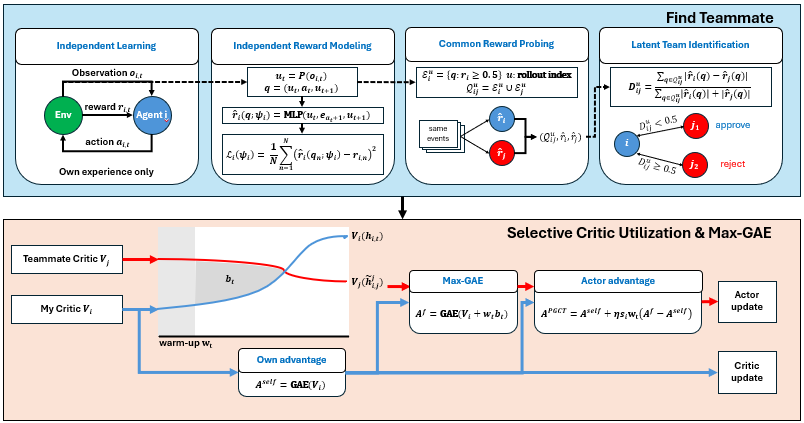
\includegraphics[width=.97\textwidth]{../figures/fig_overall.png}
\caption{에이전트 $i$의 PGCT 전체 절차. 위: 에이전트는 자기 경험으로 학습하고 공개 전이로 보상 예측기를 맞춘다. 다른 에이전트를 만나면 두 예측기가 같은 보상 사건 probe에 답하고, 응답 거리가 계속 작으면 승인한다(단순화한 그림이며 전체 규칙은 식~\ref{eq:approval}). 아래: 승인된 팀원의 Critic이 GAE의 가치 입력을 양의 상승분 $b_t$만큼 올린다. 이는 Actor update만 바꾸고, Critic은 계속 자기 return을 학습한다. 모든 계산은 각 에이전트 안에서 하며, 만났을 때만 공개 사건 view, 예측 응답, Critic 가중치를 주고받는다.}\label{fig:architecture}
\end{figure*}

그림~\ref{fig:architecture}는 PGCT의 두 부분인 팀 발견(위)과 팀원 Critic 접근(아래)을 보여 준다. 알고리즘~\ref{alg:pgct}는 update 한 번의 절차다.

\subsection{개인 보상 예측}
각 에이전트는 공개 전이 $q=(u_t,a_t,u_{t+1})$로 자기 보상을 예측하는 다층 퍼셉트론을 학습한다.
\ModelEquation
$e_{a_t+1}$은 행동의 one-hot 벡터다($e_k$는 $\mathbb R^{5}$의 $k$번째 단위벡터이고, 행동 번호는 0부터 센다). 사건은 자기 보상이 $r_i\ge0.5$인 전이다. 사건은 드물기 때문에, 각 에이전트는 최근 사건을 따로 저장하고 매 학습 batch의 일정 비율을 사건으로 채운다. batch $\{(q_n,r_{i,n})\}_{n=1}^{N}$에 대한 손실은 다음과 같다.
\RewardLossEquation
공개 view는 공개하면 안 되는 정보를 숨기므로, 같은 공개 전이가 어떤 때는 보상이고 어떤 때는 아니다. 이때 예측기는 그 전이의 기대 보상을 배우며, 우리가 비교하는 값이 바로 이것이다.

\subsection{Reward Probe}
rollout $u$ 동안 $i$와 $j$가 만났다면, 두 에이전트는 다음 공통 probe 집합을 만든다.
\ProbeEquation
$\mathcal E_i^u$는 rollout $u$가 시작되기 전 에이전트 $i$의 최근 자기 사건들의 공개 view다. 보상 값은 probe에 들어가지 않는다. 두 에이전트가 모두 보상을 받아 봤다면, 두 사건 집합에 이미 팀을 가르는 정보가 들어 있다. 한 목적지의 배송은 한 팀에게만 보상이다.

\paragraph{rollout 시작 시점 스냅샷.}
비교는 rollout이 끝난 뒤에 하지만, 두 에이전트는 rollout 초반에 만났을 수도 있다. 접촉 시점에 있던 정보만 쓰기 위해, 각 에이전트는 rollout 시작 때 사건 view, 성숙 여부, 예측기를 고정한다. 예측기는 rollout이 끝난 뒤에만 다시 학습한다. 비교는 이 고정본으로 하고, 재학습보다 먼저 한다.

\begin{figure}[t]
\centering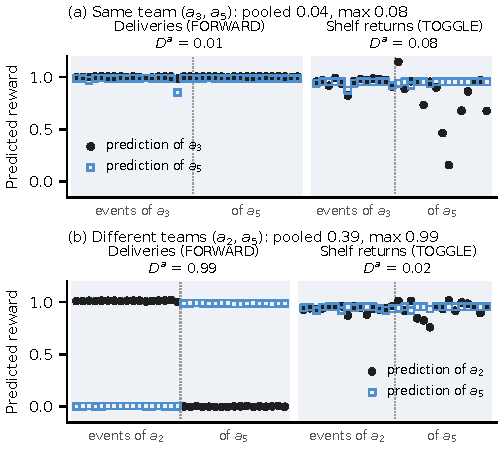
\includegraphics[width=\columnwidth]{../figures/fig_discovery_data.pdf}
\caption{공통 probe에 대한 두 에이전트의 보상 예측. 실제 학습에서 저장한 예측기로 그렸다(모서리 목적지, 개인 보상, seed 1, 4.35M step, 이전 규칙 학습, 대칭 probe 없음). probe는 각 에이전트의 최근 자기 사건 32개이며 행동별로 묶었다. (a) 같은 팀 $a_3$, $a_5$는 모든 probe에서 높은 보상을 예측한다. (b) 다른 팀 $a_2$, $a_5$는 두 팀 모두 보상받는 선반 반납에서는 예측이 같지만, 배송에서는 다르다. 합친 거리(0.39)는 문턱 0.5보다 작지만, 행동별 최댓값(0.99)은 그렇지 않다.}\label{fig:discovery}
\end{figure}

\subsection{응답 거리와 팀 발견}
두 예측기는 같은 probe를 평가한다(그림~\ref{fig:discovery}). probe를 행동별로 나눈다. $\mathcal Q_{ij}^{u,a}$는 행동이 $a$인 probe이고, $\mathcal E_i^u(a)$는 에이전트 $i$의 사건 중 행동이 $a$인 것이다. 응답 거리는 다음과 같다.
\ActionDistanceEquation
즉 두 에이전트가 모두 행동 $a$의 자기 사건을 $n_{\min}$개 이상 가졌을 때만 그 행동을 비교한다. 비교할 행동이 없으면 그 round에는 비교하지 않는다. 어떤 행동의 분모가 $10^{-8}$보다 작으면 그 행동은 건너뛴다.

삼각부등식에 의해 각 행동별 거리는 $[0,1]$ 안에 있고, 두 예측기에 같은 배율을 곱해도 변하지 않는다. 최댓값을 쓰는 이유는 다음과 같다. probe를 모두 합쳐 계산하면 거리는 $\sum_a w_aD_{ij}^{u,a}$가 된다. 여기서 $w_a\ge0$는 분모 중 행동 $a$가 차지하는 비율이고 $\sum_a w_a=1$이다. 따라서 합친 거리는 최댓값보다 클 수 없고, 예측 보상이 큰 행동일수록 가중치가 커진다. 이 과제의 선반 반납처럼 모든 팀이 보상받는 사건이 많아지면, 그 행동의 가중치가 커져 다른 행동에서의 뚜렷한 차이를 가린다(그림~\ref{fig:discovery}b). 같은 팀은 보상 규칙이 같으므로 모든 행동의 거리가 작고, 따라서 최댓값도 작다. $n_{\min}$ 조건은 거의 보상받아 본 적이 없는 사건으로 에이전트를 판단하지 않게 한다.

에이전트는 자기 사건을 20개 이상 겪었고, 예측기가 학습되었으며, 자기 최근 사건에 대한 평균 예측이 0.3 이상일 때 \emph{성숙}했다고 본다($m_i^u=1$). 쌍은 5 update마다, 두 에이전트가 모두 성숙했을 때만 비교한다. 거리는 비교 round에 걸쳐 평활하고, 쌍은 다음 규칙으로 승인한다.
\ApprovalEquation
$n_{ij}$는 새 예측기를 쓴 round의 수다. 그 쌍의 마지막 집계 이후 $\widehat r_i$나 $\widehat r_j$가 다시 학습된 경우에만 round를 센다. 다시 학습되지 않은 round는 $\bar D_{ij}$와 $n_{ij}$를 바꾸지 않는다. 승인은 대칭이다. 접촉이 끊겨도 승인은 유지되지만, 다시 만났을 때만 쓰인다. 문턱 0.5는 미리 정했다. 이 판정에는 팀 라벨을 쓰지 않는다.

발견은 두 팀의 보상 규칙이 어떤 공개 사건에서 서로 다른 예측을 낼 때만 가능하다. 행동별 거리에서는 이 차이가 두 에이전트 모두 $n_{\min}$번 이상 겪은 행동에서 나타나야 한다. 보상을 받아 본 적이 없는 에이전트는 비교할 예측이 없으므로, PGCT는 그 에이전트에 대해 판정을 보류한다.

\subsection{팀원 Critic 접근}
rollout $u$에서 에이전트 $i$의 donor 집합은 다음과 같다.
\begin{equation}\label{eq:donorset}
\mathcal G_i^u=\{j\ne i: C_{ij}^u=1,\ B_{ij}=1\}.
\end{equation}
donor Critic 가중치는 rollout $u$ 동안 쓰인 가중치이며, 만났을 때 받고 update 동안 바꾸지 않는다. 에이전트 $i$는 자기 관측 열을 각 donor Critic에 다시 넣는다. 그래서 donor의 recurrent 상태 $\tilde h^{\,j}_{i,t}$는 받는 쪽에서 계산하고, donor의 hidden 상태는 보내지 않는다. 이 재생은 rollout 시작 때 0 상태에서 시작하고 episode가 끝나면 초기화한다. 처음 몇 step의 재생 가치는 아직 믿을 수 없으므로 마스크 $w_t=0$으로 뺀다.

\subsection{Max-GAE advantage 추정}
donor 집합이 비어 있지 않으면 양의 상승분과 결합 가치는 다음과 같다.
\MaxEquation
GAE는 trainer의 episode 종료와 시간 제한 처리를 그대로 따른다.
\GAEEquation
$d_t$는 episode 종료 표시이고, $z^f_{i,t}$는 시간 제한으로 끝난 관측의 가치다(그 밖에는 0). 자기 advantage $A^{\rm self}$는 $f$ 대신 $V_i$로 같은 재귀를 계산한다. Actor advantage는 다음과 같다.
\BlendEquation
마스크 $w_t$는 $b$만이 아니라 차이 $A^f-A^{\rm self}$ 전체에 곱한다. $b$만 가리면 뒤쪽 step의 상승분이 GAE 재귀를 따라 가려진 step으로 들어올 수 있다. 계수 $s_i\le1$은 큰 보조 항을 자기 advantage 크기로 줄이지만, 작은 항을 키우지는 않는다. 이 과제에서 뒤처진 에이전트의 원래 차이는 $\operatorname{std}(A^{\rm self})$의 2.6--12배였다. $s_i$가 없으면 PPO의 advantage 정규화(식~\ref{eq:ppo}) 때문에 결과가 $\eta$와 거의 무관해진다. 승인된 donor가 없거나 모든 step에서 상승분이 0이면 $A^{\rm PGCT}=A^{\rm self}$이므로, 방법은 독립 PPO와 같아진다.

\subsection{Actor와 Critic update}
Actor는 기존 advantage $A^{\rm self}$ 대신 $A^{\rm PGCT}$로 PPO 학습을 한다. 일반 PPO처럼, 먼저 에이전트별로 rollout 전체에서 advantage를 정규화한다.
\PPOEquation
Actor는 $L_i^\pi$에 엔트로피 보너스를 더해 최대화한다. Critic은 독립 PPO와 똑같이 학습한다. Critic의 목표 $R^{\rm self}$는 $A^{\rm PGCT}$가 아니라 $A^{\rm self}$로 계산하고, Critic은 이 목표를 향한 clip된 가치 손실을 최소화한다. 따라서 팀원 Critic은 Actor update만 바꾸고, 팀원 증류 손실은 없다. Actor와 Critic은 encoder와 recurrent 층을 따로 쓴다. 다만 gradient norm clip을 함께 쓰므로, Actor advantage가 Critic step의 크기를 바꿀 수는 있지만 목표는 바꾸지 않는다.

\begin{algorithm}[tb]
\caption{에이전트 $i$의 PGCT update $u$}
\label{alg:pgct}
\begin{algorithmic}[1]
\REQUIRE Actor $\pi_{\theta_i}$, Critic $V_i$, 보상 예측기 $\widehat r_i$, 쌍 통계 $\bar D_{ij},n_{ij}$
\STATE $\mathcal E_i^u$, $m_i^u$, $\widehat r_i^{\,u}$ 고정 \COMMENT{rollout 시작 스냅샷}
\STATE $\pi_{\theta_i}$로 rollout; $(q_t,r_{i,t})$ 저장, $r_{i,t}\ge0.5$이면 사건 버퍼에 추가
\STATE 접촉 $C_{ij}^u$ 기록 \COMMENT{식~\ref{eq:donor}}
\IF{$u \bmod 5=0$}
\FOR{$C_{ij}^u=1$이고 $m_i^u=m_j^u=1$인 $j$}
\STATE $\mathcal Q_{ij}^u\leftarrow\mathcal E_i^u\cup\mathcal E_j^u$
\STATE $D_{ij}^u\leftarrow\max_{a\in\mathcal A_{ij}^u}D_{ij}^{u,a}$ \COMMENT{식~\ref{eq:distance}}
\IF{마지막으로 집계한 round 이후 $\widehat r_i$나 $\widehat r_j$가 다시 학습됨}
\STATE $\bar D_{ij}\leftarrow(1-\beta)\bar D_{ij}+\beta D_{ij}^u$,\ \ $n_{ij}\leftarrow n_{ij}+1$
\ENDIF
\STATE $B_{ij}\leftarrow\mathbf 1[n_{ij}\ge3,\ \bar D_{ij}<0.5]$ \COMMENT{식~\ref{eq:approval}}
\ENDFOR
\STATE $\mathcal L_i^r$를 최소화해 $\widehat r_i$ 재학습 \COMMENT{식~\ref{eq:rloss}}
\ENDIF
\STATE $\mathcal G_i^u\leftarrow\{j:C_{ij}^u=1,\ B_{ij}=1\}$
\STATE $b_{i,t}\leftarrow[\max_{j\in\mathcal G_i^u}V_j(\tilde h_{i,t}^{\,j})-V_i(h_{i,t})]_+$ \COMMENT{식~\ref{eq:max}}
\STATE $f_{i,t}\leftarrow V_i(h_{i,t})+w_tb_{i,t}$
\STATE $A^{f}\leftarrow\mathrm{GAE}(f)$,\ \ $A^{\rm self}\leftarrow\mathrm{GAE}(V_i)$ \COMMENT{식~\ref{eq:gae}}
\STATE $A^{\rm PGCT}_{i,t}\leftarrow A^{\rm self}_{i,t}+\eta s_iw_t(A^f_{i,t}-A^{\rm self}_{i,t})$ \COMMENT{식~\ref{eq:blend}}
\STATE $A^{\rm PGCT}$로 $\pi_{\theta_i}$, $R^{\rm self}$로 $V_i$ update \COMMENT{식~\ref{eq:ppo}}
\end{algorithmic}
\end{algorithm}

\section{실험}
\subsection{설정}\label{sec:setup}
\paragraph{환경.} 로봇 창고 환경 \citep{benchmark}의 다중 팀 변형을 쓴다. $11\times10$ 격자에 에이전트 6개가 3개씩 두 팀으로 나뉜다. 팀 목적지는 아래쪽 두 모서리 $(0,10)$과 $(9,10)$이고, 팀마다 요청 선반이 3개 있다. 관측은 감지 반경 5의 의미 격자다. 모든 에이전트는 자기 보상을 받는다. 배송 1, 선반 반납 1, 요청 선반 집기 0.15, 작은 진척 항(0.02, 0.005, 0.002), 비생산적 행동에 대한 작은 감점(0.002--0.05)이다. 팀 보상은 쓰지 않는다. 표~\ref{tab:settings}에 학습 설정을 정리했다.

\paragraph{구현.} 공개 view $P(o)$는 자기 상태 특징 6개와 반경 2 이내의 물리 격자 채널 11개(281개 값)를 남긴다. 그래서 예측기 입력은 $281+5+281=567$개 값이다. 예측기의 은닉층은 ReLU 128개와 64개다. 각 에이전트는 최근 전이 20{,}000개와, 이와 별도로 최근 사건 512개를 저장한다. 사건은 전체 전이의 0.5\% 미만이므로 batch의 4분의 1을 사건 버퍼에서 뽑는다. 예측기는 PPO update 5번마다 Adam으로 50 step 학습한다(batch 256, 학습률 $10^{-3}$). probe에는 에이전트마다 최근 사건 32개를 쓰고, $n_{\min}=8$이다. 재생 마스크는 관측 8개가 지나거나 첫 초기화가 일어날 때까지 donor 가치를 뺀다.

\paragraph{방법 버전.} 아래의 발견 결과는 이전 버전의 규칙으로 얻었다. 이전 버전은 모든 probe를 합쳐 거리를 계산했고(pooled), probe에 좌우 대칭 사본을 더했으며, $r_c=3$을 썼다. 행동별 거리로 바꾼 이유는 \ref{sec:discovery}절에 적었다. 현재 방법(행동별 거리, 대칭 사본 없음, $r_c=5$)을 더 넓은 $11\times16$ 지도에서 실행하고 있다.

\begin{table}[t]\centering\small
\begin{tabular}{ll}\toprule
설정 & 값\\\midrule
rollout / recurrent 길이 & 1024 / 64 step\\
PPO epoch / minibatch & 4 / 8\\
학습률 / 엔트로피 & $2\times10^{-4}$ / 0.05\\
PPO clip / 가치 clip & 0.2 / 0.2\\
할인율 / GAE 계수 & 0.99 / 0.95\\
encoder / GRU 폭 & 128 / 128\\
보상 학습 간격 / step & 5 update / 50\\
사건 기준 / 성숙 & $r\ge0.5$ / 사건 20개\\
에이전트당 probe 사건 / $n_{\min}$ & 32 / 8\\
EMA $\beta$ / 문턱 / round & 0.35 / 0.5 / 3\\
Max-GAE $\eta$ / 척도 & 0.5 / shrink\\
이전 실험: $r_c$ / 대칭 probe & 3 / 사용\\\bottomrule
\end{tabular}
\caption{환경 상호작용과 PGCT 설정.}\label{tab:settings}
\end{table}

\paragraph{분기 실험.} 전체 방법을 온라인으로 실행하기 위해, 1.024M step의 공통 독립 PPO checkpoint(seed 1)에서 시작해 seed 1, 3, 5로 0.5M step을 더 학습한다. 이 seed들은 checkpoint의 목적지 배치를 유지한다. 이 checkpoint에서 세 에이전트($a_0,a_1,a_4$)는 배송이 거의 없거나 전혀 없다. 대조군으로, 같은 분기에서 성숙한 에이전트로 제한한 실제 팀원을 donor로 쓰는 학습도 돌렸다. 이 학습도 같은 발견 통계를 기록한다. 분기 seed는 하나의 학습을 이어 간 것이므로 독립 학습 seed가 아니다.

\subsection{팀 발견}\label{sec:discovery}
그림~\ref{fig:gate-data}는 이전 발견 규칙으로 돌린 5M step 학습(seed 1)이다. 에이전트가 성숙하자 같은 팀과 다른 팀 쌍이 바로 갈린다. 0.1--0.25M 구간에서 평균 응답 거리는 팀원 0.25, 그 밖 0.99이고, 0.25M까지 6개 중 5개 에이전트가 성숙했다. 같은 팀 거리는 계속 내려간다(4M 이후 0.08). 다른 팀 거리는 약 1M까지 0.99 근처에 있다가 천천히 내려간다. 학습 전체에서 방향 있는 팀원 접근 arc 5{,}252개가 실제 팀원에게, 352개가 다른 팀에게 갔고, 같은 팀 비율은 93.7\%다. 첫 다른 팀 승인은 4.28M step에 나오므로, 그 전의 접근은 모두 맞았다. 이 비율은 접근 횟수를 센 값이며 쌍 단위 정확도가 아니다. 이 학습은 update 끝의 위치를 접촉으로 썼고 이전의 팀원 활용 규칙을 썼으므로, 발견 부분만 평가한다.

늦게 나타난 거리 하락의 원인을 찾았다. 두 팀 모두 선반 반납으로 보상받고, 공개 view에서 반납 장면은 두 팀에게 똑같이 보인다. 에이전트가 배송과 반납을 끝까지 하게 되면서, 활발한 에이전트의 최근 사건 32개 중 반납이 약 3개에서 약 14개로 늘었고, 두 예측기 모두 반납에 높은 보상을 예측했다. 그 결과 가장 활발한 에이전트와 다른 팀 사이의 세 쌍에서 합친 거리가 0.5 아래로 내려갔고, 이 세 쌍이 다른 팀 arc 352개를 모두 만들었다. 그래서 행동별 거리로 바꿨다. 이 학습과 분기 실험 세 개의 checkpoint 25개에서, 저장된 예측기와 probe로 두 거리를 대칭 사본 없이 오프라인으로 다시 계산했다. 행동별 거리는 모든 checkpoint에서 같은 팀이 최대 0.28, 다른 쌍이 최소 0.97이었다(그림~\ref{fig:gate-data}d). 합친 거리에서는 다른 팀 쌍 하나가 0.39까지 내려갔다.

추가 오프라인 점검으로, 끝난 독립 PPO 학습의 경험 일부(0.26--5M step, 전이의 약 1/180)를 이전 규칙에 재생했다. 모든 쌍이 매 round 접촉한다고 가정했다. 15쌍 중 판정에 이른 10쌍은 모두 맞게 분류되었다. 같은 팀 승인 4쌍, 다른 팀 승인 0쌍이다(같은 팀 거리 0.14--0.18, 다른 팀 0.58--0.70). 나머지 5쌍은 모두 배송을 끝내 배우지 못한 한 에이전트가 낀 쌍이었고, 판정을 보류했다. 이 재생에서 대칭 probe를 빼도 판정은 하나도 바뀌지 않았다.

분기 실험(\ref{sec:setup}절)은 rollout 시작 스냅샷과 접촉 규칙을 포함한 전체 방법을 온라인으로 실행한다. PGCT 분기 세 개(seed 1, 3, 5; seed 5는 0.5M 중 0.46M까지)에서 다른 팀 쌍은 한 번도 승인되지 않았고, Max-GAE가 쓴 donor arc는 모두 실제 팀원을 향했다(1{,}920, 1{,}350, 1{,}258개). 첫 승인은 분기 후 20k--26k step에 나왔다. 각 학습에서 네 에이전트가 성숙했다. 한 팀의 세 에이전트 전부와 다른 팀의 한 에이전트다. PGCT는 첫 팀 안의 방향 있는 arc 6개를 모두 승인했다. 혼자 성숙한 에이전트와 그 팀 사이의 arc 6개는 하나도 승인하지 않았다. 따라서 같은 팀 arc 12개 중 6개를 찾았고 나머지는 판정을 보류했다. 대조군 세 학습에도 다른 팀 승인은 없다. 이 분기는 학습 1.02--1.52M step 구간으로, 5M 학습 후반의 다른 팀 거리 하락보다 앞선다.

\begin{figure*}[t]\centering
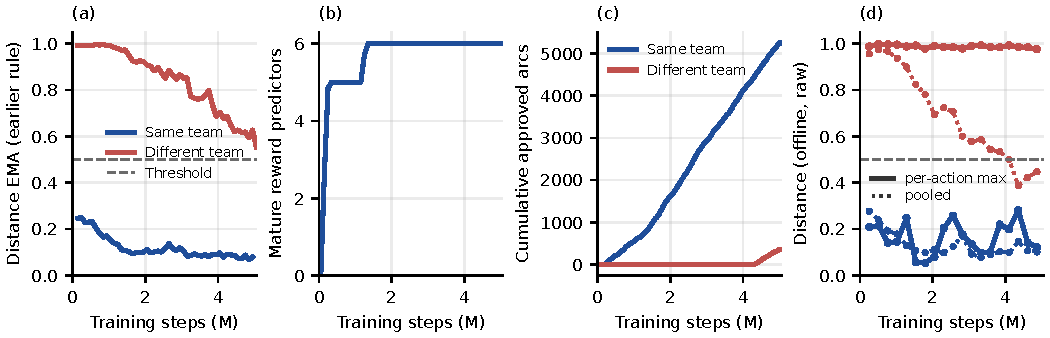
\includegraphics[width=.98\textwidth]{../figures/discovery_log_v2.pdf}
\caption{창고 과제의 팀 발견(모서리 목적지, 개인 보상, seed 1, 5M step). (a)--(c)는 이전 규칙(합친 거리, 대칭 probe, $r_c=3$)의 학습 로그다. (a) 비교한 쌍의 응답 거리 EMA 평균, 100k step 구간. 점선은 승인 문턱이다. (b) 보상 예측기가 성숙한 에이전트 수. (c) 실제 관계별 방향 있는 팀원 접근 arc 누적. (d) 모든 checkpoint의 저장된 예측기와 probe로 대칭 사본 없이 오프라인에서 다시 계산한 거리. 같은 팀의 최댓값(파랑)과 다른 팀의 최솟값(빨강)을 행동별 최댓값(실선)과 합친 거리(점선)로 나타냈다.}\label{fig:gate-data}
\end{figure*}

\subsection{팀 관계가 팀원 가치에 중요한 이유}
\begin{figure}[t]
\centering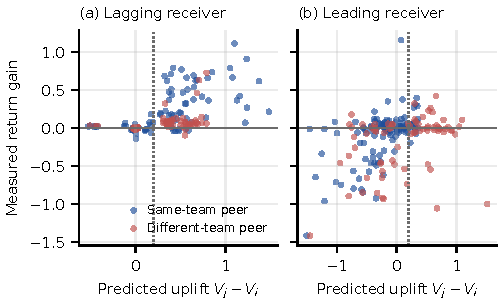
\includegraphics[width=\columnwidth]{../figures/counterfactual.pdf}
\caption{저장된 독립 PPO checkpoint(데이터 네 묶음)에서 한 반사실 점검. 여기서는 Max-GAE로 학습한 에이전트가 없다. Max-GAE가 더할 상승분이 실제 이득과 맞는지를 확인한다. 점 하나가 받는 에이전트의 상태 하나다. 가로축은 팀원 Critic이 받는 에이전트에 대해 예측한 상승분 $V_j-V_i$, 세로축은 받는 에이전트가 그 팀원의 정책으로 움직였을 때 100 step 동안 실제로 바뀐 자기 return이다(공통 난수, 8회 반복). (a) 뒤처진 에이전트. (b) 앞선 에이전트. 점선은 상승분 0.2다.}\label{fig:cf}
\end{figure}

팀원의 Critic이 다른 팀의 Critic보다 더 쓸모 있는지 확인했다. 저장된 독립 PPO checkpoint를 썼다. 한 학습의 두 시점과, 좌표가 보이는 이전 설정의 두 학습이다. 같은 환경 상태에서 받는 에이전트를 자기 정책으로, 또는 다른 에이전트의 정책으로 움직이게 했고, 나머지 에이전트는 자기 정책을 유지했다. 그리고 받는 에이전트의 return 변화를 팀원 Critic이 예측한 상승분과 비교했다(그림~\ref{fig:cf}). 예측 상승분이 0.2보다 큰 뒤처진 에이전트에서, 같은 팀 정책은 56번 중 89\%에서 return을 높였고 평균 이득은 0.36이었다. 비슷한 예측 상승분의 다른 팀 정책은 평균 0.10에 그쳤다. 앞선 에이전트에서는 0.2보다 큰 다른 팀 상승분의 평균 변화가 $-0.04$였고, 절반만 return을 높였다. 예측 상승분은 실제 이득보다 최대 1.6배 컸다. 이 결과는 발견 단계와 상승분 크기 조정이 모두 필요하다는 근거다.

\section{결론}
PGCT는 개인 보상 응답으로 잠재 팀원을 온라인에서 찾는다. 각 에이전트는 자기 보상을 예측하고, 만난 에이전트와 공개 보상 사건에서 예측을 행동별로 비교하며, 충분한 자기 경험이 있을 때 반복된 일치만 승인한다. 승인된 팀원의 Critic은 마스크와 크기 조정을 둔 Max-GAE 항으로 Actor advantage를 바꾸고, 각 Critic은 자기 return을 유지한다. 두 팀 창고 과제에서 발견은 이른 시점에 팀원을 구분했고 팀원 접근의 대부분을 실제 팀원에게 보냈다. 전체 방법의 분기 실험에서는 다른 팀 쌍을 한 번도 승인하지 않았다. 이 접근이 학습을 빠르게 하는지는 아직 검증 중이다.

\bibliographystyle{plainnat}
\bibliography{../references}

\appendix
\section{구현 세부}
발견 상태의 일관성을 검사한다. rollout 시작 스냅샷과 비교 사이에 예측기가 다시 학습되면 오류로 처리한다. 승인은 저장된 round와 EMA 값에서 다시 구성하며, 고정된 성숙 표시와 대조한다. 행동별 거리에서 probe는 공개 행동으로 묶는다. 에이전트마다 고정된 사건 32개 중 그 행동의 사건이 $n_{\min}=8$개 이상일 때만 그 행동을 비교하고, 비교할 행동이 없으면 그 round를 건너뛰며 EMA와 round 수를 바꾸지 않는다. 자기 rollout에서 explained variance가 문턱보다 낮은 donor Critic을 빼는 선택 필터가 있지만, 문턱을 정하지 않았으므로 꺼 두었다. donor 집합은 update 한 번 동안 고정된다. 자기 return 목표는 Actor advantage를 만들기 전에 계산한다.

근거 자료: 발견 로그는 \path{runs/acv2_s1_20261029_084340}, 분기 실험은 \path{runs/pgctd2_br1M_20261102_180212}(W\&B 요약: \path{output/branch_wandb_20261104})이다. 행동별 거리의 오프라인 재계산은 \path{output/ac_drift_20261104}에 있다. 그림 3은 원본 로그에서 \path{output/pgct_docs_20261102/evidence_plots.py}로, 그림 2는 \path{output/pgct_docs_20261102/discovery_illustration.py}로 다시 만든다.
\end{document}
